% EEE3096S Practical 1B report, Group 79

\documentclass[11pt]{article}
\usepackage{hyperref}
\usepackage{graphicx}
\usepackage[a4paper, margin=2.5cm]{geometry}
\usepackage{amsmath}
\usepackage{booktabs}
\usepackage{listings}
\usepackage{xcolor}
\usepackage{float}
\usepackage{placeins}

% every remaining bench measurement is wrapped in this so nothing unfilled
% can be mistaken for a result
\newcommand{\bench}[1]{\textcolor{red}{\textbf{[BENCH: #1]}}}

% figure slot for a screenshot that is not taken yet. drop the file into
% figures/ under the name below and it appears, no edit needed
\newcommand{\scopefig}[3]{%
  \begin{figure}[h]
  \centering
  \IfFileExists{figures/#1}{%
    \includegraphics[width=0.85\linewidth]{figures/#1}%
  }{%
    \fbox{\parbox[c][45mm][c]{0.85\linewidth}{\centering
      \textcolor{red}{\textbf{[BENCH] figures/#1 not captured yet}}}}%
  }
  \caption{#3}
  \label{fig:#2}
  \end{figure}%
}

\lstset{
  basicstyle=\ttfamily\footnotesize,
  breaklines=true,
  frame=single,
  columns=fullflexible,
  keepspaces=true,
}

\title{\textbf{EEE3096S Practical 1B} \\ Execution Timing and Cycle-Accurate Assembly on the UCT Dev Board}
\author{Tri Tac Le, LXXTRI004 \\ Gil Sharon, SHRGIL004}
\date{\today}

\begin{document}

\maketitle

\section{Golden Measure and PC Timing}

\subsection{The function under test}

The quantity computed throughout this practical is the integer square root of a
32-bit unsigned input $x$, defined as the largest integer $r$ satisfying
$r^2 \le x$. The golden version uses double precision arithmetic and the
standard library \texttt{sqrt}. The result is then checked and adjusted to ensure its square is not greater than the input, and that the following integer's square is greater than the input. 

\begin{lstlisting}[language=C]
uint32_t isqrt_golden(uint32_t x) {
  uint32_t r = (uint32_t)sqrt((double)x);
  while ((uint64_t)r * r > (uint64_t)x) r--;
  while ((uint64_t)(r + 1) * (r + 1) <= (uint64_t)x) r++;
  return r;
}
\end{lstlisting}
\noindent
This correction matters for values which may be rounded up. A \texttt{double} holds 53 significand bits,
so every 32-bit input is represented exactly, but a square root of a value which is just below a perfect square can round up to the next integer and give an answer one too large. Both loops together make the returned value correct by construction
rather than correct by assumption.

\subsection{Prediction before timing}

The prediction was made from an instruction count estimate before the timing
run. The host is an Apple MacBook Air with an Apple M1, four
performance cores and four efficiency cores. A performance core runs at about
3.2 GHz, so one clock cycle is about 0.3125 ns.
\noindent
One call performs a single hardware double-precision square root, one
conversion back to integer, and two multiply-and-compare pairs (for ensuring the values are clamped correctly),
of which neither loop body executes in the common case. Taking an effective
cost of about 10 cycles per call gives

\[
t_{\text{pred}} \approx 10 \times \frac{1}{3.2 \times 10^{9}~\text{Hz}}
= 10 \times 0.3125~\text{ns} \approx 3.1~\text{ns per call}.
\]
\noindent
As a result, the prediction is therefore about 3.1 ns per call.

\subsection{Measured results}
The execution time was measured through
\texttt{clock\_gettime(CLOCK\_MONOTONIC, \ldots)}, which is called before and after the test loop,
whose input changes on every iteration. Each calculated result was written to a
\texttt{volatile} variable so that the compiler would not remove the calculations during optimisation. The program was
built with \texttt{gcc -O2 -std=gnu11}.

\begin{table}[h]
\centering
\begin{tabular}{lrr}
\toprule
Run & Repetitions & Time per call (ns) \\
\midrule
A & 1\,000\,000 & 2.959 \\
B & 10\,000\,000 & 2.517 \\
\midrule
\multicolumn{2}{l}{Mean} & 2.738 \\
\multicolumn{2}{l}{Spread} & 0.442 (16.15\% of mean) \\
\bottomrule
\end{tabular}
\caption{Golden measure timing on the PC, two repetition counts.}
\label{tab:pc-timing}
\end{table}
\noindent
The two runs differ by 0.442 ns, which is 16.15\% of the mean. This difference is likely caused by normal variation in short execution-time measurements, including processor frequency changes (modern processors change frequency dynamically), operating-system scheduling, and other background activity. The 1,000,000 repetition test completes in only a few milliseconds, making it more sensitive to these short-term effects. The 10,000,000 repetition test runs for longer and therefore averages these effects over a greater number of calculations, making its measured time more representative. 
\noindent
The mean of 2.738 ns sits close below the 3.1 ns predicted. The prediction
assumed roughly 10 cycles of work per call at 3.2 GHz. The measurement coming
in slightly under that could mean that the the CPU may be working on several loop iterations at once rather than completely finishing one before beginning the next.

\subsection{Output table for the ten inputs}

\begin{table}[h]
\centering
\begin{tabular}{rrrrl}
\toprule
Input $x$ & $r$ & $r^2$ & $(r+1)^2$ & Check \\
\midrule
0 & 0 & 0 & 1 & pass \\
1 & 1 & 1 & 4 & pass \\
15 & 3 & 9 & 16 & pass \\
16 & 4 & 16 & 25 & pass \\
4095 & 63 & 3969 & 4096 & pass \\
65535 & 255 & 65025 & 65536 & pass \\
123456789 & 11111 & 123454321 & 123476544 & pass \\
987654321 & 31426 & 987593476 & 987656329 & pass \\
4294836225 & 65535 & 4294836225 & 4294967296 & pass \\
4294967295 & 65535 & 4294836225 & 4294967296 & pass \\
\bottomrule
\end{tabular}
\caption{Golden outputs with the squares for every input.}
\label{tab:golden}
\end{table}

\subsection{Hand check written out in full}

Take $x = 987654321$ with the reported result $r = 31426$.

\begin{align*}
r^2 &= 31426^2 = 31426 \times 31426 \\
    &= 987\,593\,476.
\end{align*}

Since $987\,593\,476 \le 987\,654\,321$, the value $r$ does not overshoot. Now
the next integer:

\begin{align*}
(r+1)^2 &= 31427^2 \\
&= 987\,656\,329.
\end{align*}

\noindent
Since $987\,656\,329 > 987\,654\,321$, no larger integer qualifies. The two
inequalities together prove $\mathrm{isqrt}(987654321) = 31426$.

\subsection{Task 1 question}

The golden output for the input 987654321 is \textbf{31426}. The measured time
per call is \textbf{2.959 ns} in run A and \textbf{2.517 ns} in run B, using
\textbf{1\,000\,000} and \textbf{10\,000\,000} repetitions respectively.
\noindent
A single call timed on its own is not reliable because the quantity being
measured is quicker than the tools used to measure it. One call takes about three
nanoseconds while \texttt{clock\_gettime} itself costs tens of nanoseconds, so
the clock call would dominate the reading. On top of that, the first call runs
with a cold branch predictor and cold caches, the core may still be at a low
clock frequency, and the scheduler can preempt at any point. Averaging over
millions of repetitions accounts for all of those one-off costs.

\clearpage
\section{Board Implementation and Timer Measurement}

\subsection{Fast implementation}

The version flashed on the board avoids floating point entirely, since the Cortex-M0 has
neither an FPU nor a hardware divider. It implements the digit-by-digit
restoring square root: two bits of the input shift into the remainder on each
pass, and sixteen passes cover the full 32-bit range.

\begin{lstlisting}[language=C]
static uint32_t isqrt_fast(uint32_t n) {
  uint32_t root = 0U, rem = 0U;
  for (int i = 0; i < 16; i++) {
    rem = (rem << 2) | (n >> 30);
    n <<= 2;
    root <<= 1;
    if (rem > root) {
      rem -= root + 1U;
      root += 2U;
    }
  }
  return root >> 1;
}
\end{lstlisting}

\noindent
Before it went into firmware the routine was checked on the PC against
\texttt{isqrt\_golden} over 21\,245\,185 values: every input from 0 to
$2^{20}$ exhaustively, every perfect square from $0^2$ to $65535^2$ together
with its two neighbours, and 20 million pseudo-random 32-bit values. There were
zero mismatches.

\noindent
On the board the same ten golden values from Table~\ref{tab:golden} are
compiled into the flashed code and compared at start-up. The LED on PB1 lights when all
ten match and the LED on PB0 lights on any failure, so the pass or fail state
is visible before any timing number is read.

\noindent
Observed result: the PB1 LED lit and the PB0 LED stayed dark, so all ten golden
values matched. The debugger confirms it directly, with
\texttt{verify\_failures} reading 0. 

\noindent
The restoring algorithm is particularly well suited to the Cortex-M0 architecture because each of its 16 iterations uses only 32-bit shifts, comparisons, additions, and subtractions, which translate into compact machine instructions. As a result, this algorithm achieved a substantially lower mean execution time than a binary-search implementation that uses 64-bit multiplication. Even though an integer square root can also be calculated using binary search in approximately 16 iterations, that method must square a candidate value during every iteration. If this calculation uses 64-bit arithmetic, the Cortex-M0 compiler generates a call to the software multiplication routine \texttt{\_\_aeabi\_lmul}, since the processor cannot complete the full 64-bit multiplication in a single instruction. This considerably increases the cost of each iteration. Inspection of the generated Cortex-M0 machine code showed that the restoring implementation occupied only 42 bytes, compared with 80 bytes for a representative binary-search implementation containing software-assisted multiplication. The restoring method can therefore provide a substantial speed advantage because of its lower cost per iteration, rather than because it performs fewer iterations.

\clearpage

\begin{figure}[!ht]
\centering
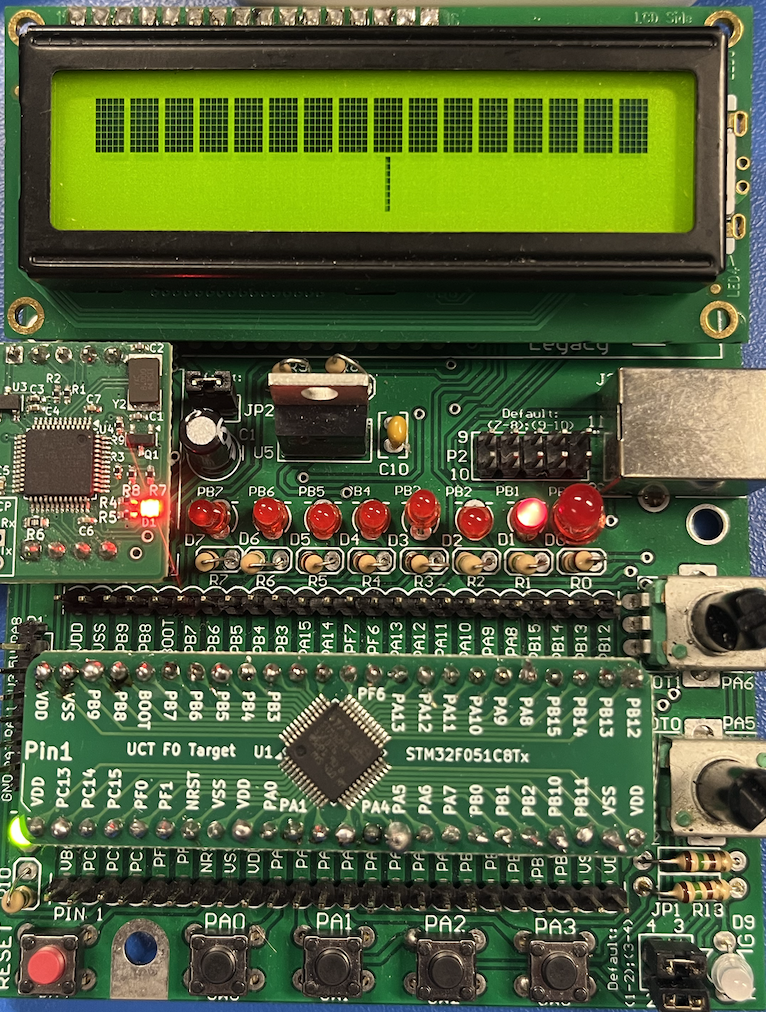
\includegraphics[height=0.42\textheight,keepaspectratio]
    {figures/task2-board-leds.png}
\caption{The board after the golden check. The LED on PB1 is lit and the LED
on PB0 is dark, which is the pass indication.}
\label{fig:leds}
\end{figure}

\begin{figure}[!ht]
\centering
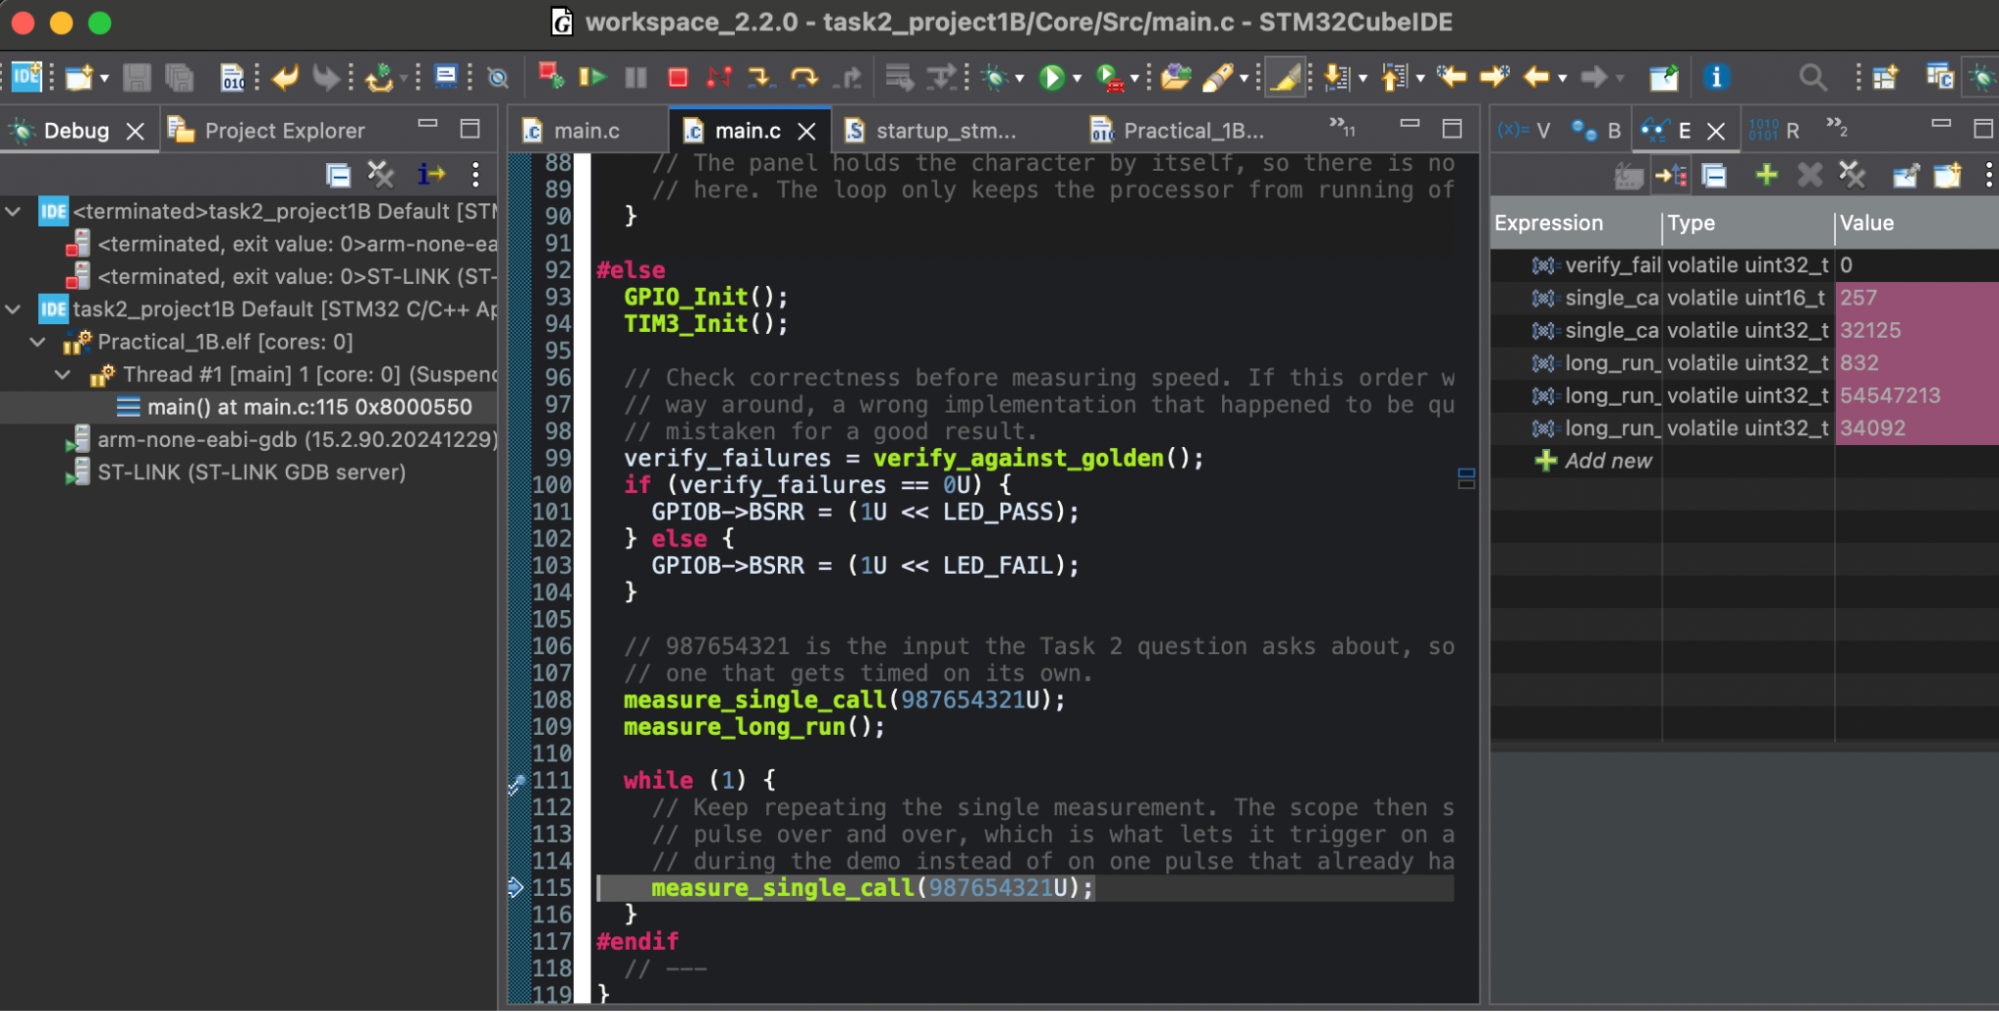
\includegraphics[width=0.90\linewidth]
    {figures/task2-debugger.png}
\caption{Debugger expression view after the run.}
\label{fig:debugger}
\end{figure}

\clearpage

\subsection{Clock path}
\noindent
The system runs from the reset configuration: HSI at 8 MHz feeding SYSCLK
directly, AHB prescaler 1, APB prescaler 1. No PLL is enabled. TIM3 sits on
APB1, and because the APB1 prescaler is 1 the timer clock equals PCLK1 at
8 MHz. The timer is then configured with

\begin{align*}
\text{PSC} &= 0 \quad \Rightarrow \quad
f_{\text{cnt}} = \frac{8\,\text{MHz}}{0 + 1} = 8~\text{MHz}, \\
\text{ARR} &= 65535 \quad \Rightarrow \quad
T_{\text{wrap}} = \frac{65536}{8 \times 10^{6}} = 8.192~\text{ms},
\end{align*}
\noindent
so one counter tick is $1/8\,\text{MHz} = 125$ ns.
\noindent
Reference manual sections used: RM0091 Section 6 for the clock tree from HSI
through SYSCLK and the APB prescalers, and RM0091 Section 18 (general-purpose
timers TIM2 and TIM3) for CNT, PSC, ARR and the update flag UIF.

\subsection{Prediction before running}

The firmware for this task was built at \texttt{-Og}, which applies
optimisation while keeping the code debuggable. \texttt{isqrt\_fast} runs a
loop of exactly sixteen passes. Each pass was estimated at about fifteen clock
cycles for the shifts, the logical operation, the comparison, the conditional
arithmetic and the loop control, giving

\[
16 \times 15 \approx 240~\text{cycles}.
\]
\noindent
A further ten cycles were allowed for function entry, initialisation and
return, for a predicted total of about 250 cycles. The CPU and the TIM3 counter
both run at 8 MHz, so one CPU cycle and one timer count are each 0.125 $\mu$s.
The prediction was therefore a count span of about 250 ticks and an execution
time of about 31.25 $\mu$s.

\subsection{Measurement}

PC13 idles high and is driven low for the timed section, so the low part of the
trace is exactly the execution window. The counter is sampled immediately
inside the low window on both sides.

\begin{lstlisting}[language=C]
GPIOC->BRR = (1U << PULSE_PIN);
uint16_t before = (uint16_t)TIM3->CNT;
sink = isqrt_fast(x);
uint16_t after = (uint16_t)TIM3->CNT;
GPIOC->BSRR = (1U << PULSE_PIN);
single_call_span = (uint16_t)(after - before);
\end{lstlisting}
\noindent
Subtracting two \texttt{uint16\_t} values handles a wrap on its own. If the
counter passes 65535 during the call, the modulo-$2^{16}$ arithmetic of the
subtraction still returns the true span, because the span is far shorter than
one 8.192 ms counter period.

\begin{itemize}
  \item Input used for the single-call measurement: 987\,654\,321
  \item Measured count span for one call: 257 ticks
  \item Time from the span: $257 \times 125$ ns = 32.125 $\mu$s
  \item Scope pulse width on PC13: 32.800 $\mu$s
  \item Difference: $32.800 - 32.125 = 0.675$ $\mu$s, or 2.10\%
\end{itemize}
\noindent
Figure~\ref{fig:pulse} shows the pulse. The cursor delta on the screen and the
time worked out from the counter span above are the same measurement taken two
different ways, so they have to agree inside the reading tolerance of the
scope.

\scopefig{task2-single-call.png}{pulse}{One call to \texttt{isqrt\_fast} at
\texttt{-Og}. PC13 is driven low for the timed section, cursors on the falling
and the rising edge give the pulse width.}

\subsection{Wrap-around case}
For the long run the firmware calls the function 200\,000 times, which at the
predicted single-call time crosses the 8.192 ms wrap several hundred times. The
update flag is polled inside the loop and counted, so the total is

\[
\text{ticks} = 65536 \times N_{\text{overflow}} + \left( \text{after} - \text{before} \right) \bmod 2^{16},
\]

and the mean per call is that total divided by 200\,000, times 125 ns.

\begin{itemize}
  \item Overflows counted: 832
  \item Residual span after the last wrap: 21\,261 ticks
  \item Total ticks: $832 \times 65\,536 + 21\,261 = 54\,525\,952 + 21\,261
        = 54\,547\,213$
  \item Total time: $54\,547\,213 \times 0.125$ $\mu$s $= 6\,818\,401.625$ $\mu$s
  \item Mean time per call: $6\,818\,401.625 / 200\,000 = 34.092$ $\mu$s
\end{itemize}
\noindent
The long-run mean of 34.092 $\mu$s is 1.967 $\mu$s higher than the 32.125 $\mu$s
measured for a single call, a difference of 6.1\%. The two numbers are not
measuring quite the same thing. The single-call span covers only the call
itself, between two adjacent reads of the counter. The long-run mean divides the
whole loop by the call count, so it also carries the per-iteration loop control,
the poll of the update flag that counts the overflows, and the update of the
input value. Those costs sit outside the single-call window and inside the long
run, which is the expected direction and roughly the expected size for a handful
of extra instructions per iteration.

\begin{itemize}
  \item Agreement with the single-call time: consistent once the per-iteration
        loop overhead described above is accounted for. The long-run figures above are read from the debugger in
Figure~\ref{fig:debugger}.
\end{itemize}


\subsection{Answer to the Task 2 question}

Scope pulse width for one call: 32.800 $\mu$s, count span 257 ticks. The
calculation from the divider values is

\[
\text{SYSCLK} = f_{\text{HSI}} = 8~\text{MHz}, \quad
\text{HCLK} = \frac{8~\text{MHz}}{1} = 8~\text{MHz}, \quad
\text{PCLK1} = \frac{8~\text{MHz}}{1} = 8~\text{MHz},
\]
\noindent
so the TIM3 counter clock is 8 MHz. With PSC = 0 the timer division factor is 1,
one count lasts $1 / (8 \times 10^{6}) = 0.125$ $\mu$s, and

\[
t = \frac{\text{span} \times (\text{PSC}+1)}{f_{\text{HSI}}}
  = \frac{257 \times 1}{8 \times 10^{6}} = 32.125~\mu\text{s}.
\]
\noindent
The counter-derived
32.125 $\mu$s and the scope pulse width of 32.800 $\mu$s differ by 0.675 $\mu$s,
which is 2.10\% of the counter figure. Because PSC is 0 and both the AHB and
APB1 dividers are 1, one timer count is exactly one CPU cycle, so the counter
time can only land on the scope reading if the clock really is 8 MHz. A
systematic error in the clock frequency would show up as a proportional gap
between the two, and 2.10\% can potentially be attributed to the combined tolerance of the HSI factory
trim and the cursor placement.


\clearpage
\setlength{\parindent}{0pt}
\section{Optimisation Flags}

\subsection{Method}

The same source was built four times with only the optimisation flag changed,
using separate build directories so no object file was reused:

\begin{lstlisting}[language=bash]
make TASK=2 OPT=-O0 BUILD_DIR=build_O0
make TASK=2 OPT=-O1 BUILD_DIR=build_O1
make TASK=2 OPT=-O2 BUILD_DIR=build_O2
make TASK=2 OPT=-Os BUILD_DIR=build_Os
\end{lstlisting}
\noindent
Sizes come from \texttt{arm-none-eabi-size} on the resulting ELF, and the
per-function sizes from \texttt{arm-none-eabi-nm --size-sort -S}. Toolchain:
arm-none-eabi-gcc 16.2.0, newlib-nano, debug information enabled in all four
builds so the comparison is like for like.

\subsection{Prediction before the -O2 build}

The \texttt{-O0} build keeps every local variable in a stack slot and reloads it
on each use, so the loop body is dominated by \texttt{ldr} and \texttt{str}
pairs which cost two cycles each. Optimised code keeps the same variables in
registers. Counting the two disassemblies gives roughly 25 memory-touching
instructions per pass at \texttt{-O0} against about 8 register operations at
\texttt{-O1} and above, so a ratio of about \textbf{2} between the \texttt{-O0}
time and the \texttt{-O2} time was predicted.

\subsection{Results}

\begin{table}[H]
\centering
\begin{tabular}{lrrrrr}
\toprule
Flag & Text (bytes) & Count span & Counter time ($\mu$s) & Scope width ($\mu$s) & Ratio to -O0 \\
\midrule
-O0 & 2080 & 753 & 94.125 & 96.000 & 1.000 \\
-O1 & 1672 & 256 & 32.000 & 33.000 & 2.941 \\
-O2 & 1848 & 246 & 30.750 & 32.200 & 3.061 \\
-Os & 1700 & 259 & 32.375 & 33.200 & 2.907 \\
\bottomrule
\end{tabular}
\caption{Optimisation level against code size and execution time. Ratios are
taken on the counter time against the \texttt{-O0} row.}
\label{tab:opt}
\end{table}

Each row of Table~\ref{tab:opt} has its own screenshot. Figure~\ref{fig:o0} is the \texttt{-O0}
baseline, Figure~\ref{fig:o1} the \texttt{-O1} build, Figure~\ref{fig:o2} the
\texttt{-O2} build and Figure~\ref{fig:os} the \texttt{-Os} build. The pulse
width read off each screen is the value in the scope column of the table.

The size column is not monotonic. At \texttt{-O1} and \texttt{-Os} the function
survives as a callable symbol and there is one copy of its body in the image. At
\texttt{-O2} there is no \texttt{bl} to \texttt{isqrt\_fast} at the call site
at all, because the compiler inlined the body into each caller, so the body is
duplicated once per call site. That is why \texttt{-O2} produces an image 176
bytes larger than \texttt{-O1} despite being the more aggressive level.
\texttt{-Os} sits between the two: it declines the transformations that trade
size for speed, and it came out 28 bytes larger and 0.375 $\mu$s slower than
\texttt{-O1} on this program. Optimising for size does not guarantee the
smallest image for every individual program, because each level enables a
different combination of transformations.

\FloatBarrier

\scopefig{task3-O0.png}{o0}{PC13 pulse width at \texttt{-O0}, the baseline that
ratios are taken against.}
\FloatBarrier

\scopefig{task3-O1.png}{o1}{PC13 pulse width at \texttt{-O1}.}
\FloatBarrier

\scopefig{task3-O2.png}{o2}{PC13 pulse width at \texttt{-O2}, the build where
\texttt{isqrt\_fast} is inlined at every call site.}
\FloatBarrier

\scopefig{task3-Os.png}{os}{PC13 pulse width at \texttt{-Os}.}
\FloatBarrier

\clearpage
\subsection{Disassembly at -O2 and the transformation identified}

The transformation is \textbf{function inlining}, applied to
\texttt{isqrt\_fast} at every call site in \texttt{main}. The source lines it
acts on are the body of \texttt{isqrt\_fast} in
\texttt{Core/Src/main.c}, and the call sites are the loop inside
\texttt{verify\_against\_golden}, the timed call inside
\texttt{measure\_single\_call} and the loop inside \texttt{measure\_long\_run}.
\noindent
At \texttt{-O0} the routine is a separate function whose locals all live on the
stack, reached through a \texttt{bl} at each call site.
The listing below is \texttt{arm-none-eabi-objdump -d} of a fresh
\texttt{-O0} build of the same source, so the addresses match the measured
image.

\begin{lstlisting}
080002fc <isqrt_fast>:
 80002fc:	b580      	push	{r7, lr}
 80002fe:	b086      	sub	sp, #24
 8000300:	af00      	add	r7, sp, #0
 8000302:	6078      	str	r0, [r7, #4]
 8000304:	2300      	movs	r3, #0
 8000306:	617b      	str	r3, [r7, #20]
 8000308:	2300      	movs	r3, #0
 800030a:	613b      	str	r3, [r7, #16]
 800030c:	2300      	movs	r3, #0
 800030e:	60fb      	str	r3, [r7, #12]
 8000310:	e01a      	b.n	8000348 <isqrt_fast+0x4c>
 8000312:	693b      	ldr	r3, [r7, #16]
 8000314:	009a      	lsls	r2, r3, #2
 8000316:	687b      	ldr	r3, [r7, #4]
 8000318:	0f9b      	lsrs	r3, r3, #30
 800031a:	4313      	orrs	r3, r2
 800031c:	613b      	str	r3, [r7, #16]
 800031e:	687b      	ldr	r3, [r7, #4]
 8000320:	009b      	lsls	r3, r3, #2
 8000322:	607b      	str	r3, [r7, #4]
 8000324:	697b      	ldr	r3, [r7, #20]
 8000326:	005b      	lsls	r3, r3, #1
 8000328:	617b      	str	r3, [r7, #20]
 800032a:	693a      	ldr	r2, [r7, #16]
 800032c:	697b      	ldr	r3, [r7, #20]
 800032e:	429a      	cmp	r2, r3
 8000330:	d907      	bls.n	8000342 <isqrt_fast+0x46>
 8000332:	693a      	ldr	r2, [r7, #16]
 8000334:	697b      	ldr	r3, [r7, #20]
 8000336:	1ad3      	subs	r3, r2, r3
 8000338:	3b01      	subs	r3, #1
 800033a:	613b      	str	r3, [r7, #16]
 800033c:	697b      	ldr	r3, [r7, #20]
 800033e:	3302      	adds	r3, #2
 8000340:	617b      	str	r3, [r7, #20]
 8000342:	68fb      	ldr	r3, [r7, #12]
 8000344:	3301      	adds	r3, #1
 8000346:	60fb      	str	r3, [r7, #12]
 8000348:	68fb      	ldr	r3, [r7, #12]
 800034a:	2b0f      	cmp	r3, #15
 800034c:	dde1      	ble.n	8000312 <isqrt_fast+0x16>
 800034e:	697b      	ldr	r3, [r7, #20]
 8000350:	085b      	lsrs	r3, r3, #1
 8000352:	0018      	movs	r0, r3
 8000354:	46bd      	mov	sp, r7
 8000356:	b006      	add	sp, #24
 8000358:	bd80      	pop	{r7, pc}
	...
\end{lstlisting}

At \texttt{-O2} there is no such symbol. The loop appears inline in the caller,
with every value held in a register and no stack traffic at all:

\begin{lstlisting}
191  rem = (rem << 2) | (n >> 30);
08000428: lsrs    r5, r0, #30
0800042a: lsls    r1, r1, #2
0800042c: orrs    r1, r5

192  n <<= 2;
0800042e: lsls    r0, r0, #2

193  root <<= 1;
08000430: lsls    r3, r3, #1

198  if (rem > root) {
08000432: cmp     r1, r3
08000434: bls.n   0x800043c

199  rem -= root + 1U;
08000436: subs    r1, r1, r3
08000438: subs    r1, #1

200  root += 2U;
0800043a: adds    r3, #2

188  for (int i = 0; i < 16; i++) {
0800043c: subs    r2, #1
0800043e: cmp     r2, #0
08000440: bne.n   0x8000428

205  return root >> 1;
08000448: lsrs    r3, r3, #1

236  sink = isqrt_fast(measured_x);
0800044a: str     r3, [r6, #0]

238  uint16_t after = (uint16_t)TIM3->CNT;
0800044c: ldr     r3, [r5, #36]
\end{lstlisting}

There is no \texttt{bl isqrt\_fast} instruction at the call site. The shift,
comparison, conditional arithmetic and loop instructions from the function body
appear directly inside the calling code instead. The transformation acts on the
call to \texttt{isqrt\_fast} on line 236 and on the function body on lines 184
to 206. Inlining removes the call and return overhead and lets the compiler
optimise the body together with the surrounding timing code.

\subsection{Trade-off between time and code size}

Inlining removes the call, the return and the argument shuffling, and it lets
the compiler specialise each copy for its call site. One copy of
the body per call site explains the 176 extra bytes the image gained between
\texttt{-O1} and \texttt{-O2}. Put the other way round, \texttt{-O2} traded
1.250 $\mu$s of execution time for 176 bytes of flash. On a part with 64 kB of
flash that is affordable, but the general shape holds: \texttt{-O2} trades speed
with space, \texttt{-Os} refuses that trade and keeps a single shared copy, and
\texttt{-O1} lands close to \texttt{-Os} in size because it does the cheap
register allocation work without the code duplication. \texttt{-O0} is worse on
both axes at once, at 2080 bytes and 94.125 $\mu$s, because the stack traffic it
emits costs cycles and bytes together.

\subsection{Answer to the Task 3 question}

Measured time at \texttt{-O0}: 94.125 $\mu$s. At \texttt{-O2}: 30.750 $\mu$s.
The measured ratio is

\[
\frac{94.125}{30.750} = 3.061,
\]

against a predicted ratio of 2.0, so the gain from optimisation was larger than
expected. The prediction only counted the saving from holding variables in
registers instead of stack slots. Two further effects were not in it. Inlining
removed the call and return overhead entirely, which the prediction had assumed
would remain. Beyond that, \texttt{-O0} builds and tears down a stack frame on
every call and reloads each local on every use, so its cost per pass is higher
than a plain instruction count suggests. Together these push the real ratio
above the predicted one.

The transformation identified in the disassembly is function inlining, acting on
the body of \texttt{isqrt\_fast} in \texttt{Core/Src/main.c}, lines 184 to 206,
at the call site on line 236 and at its other call sites in
\texttt{verify\_against\_golden} and \texttt{measure\_long\_run}.

\clearpage
\section{Cycle-Counted Phase Delay}

\subsection{Derivation of the target}

The input is a 1 kHz sine, so

\[
T = \frac{1}{f} = \frac{1}{1000} = 1~\text{ms},
\qquad
\Delta t = \frac{45^{\circ}}{360^{\circ}} T = \frac{1}{8} \times 1~\text{ms} = 125~\mu\text{s}.
\]

At the default 8 MHz HSI one CPU cycle is 125 ns, so

\[
N_{\text{cycles}} = \frac{125~\mu\text{s}}{125~\text{ns}} = 1000~\text{cycles}.
\]

\subsection{Cycle budget}

Cortex-M0 instruction costs used: \texttt{MOVS}, \texttt{SUBS} and \texttt{NOP}
one cycle; \texttt{LDR} and \texttt{STR} two cycles; a branch three cycles when
taken and one when it falls through.

The path that must add up to 1000 cycles runs from the sample instant to the
DAC write. The sample and hold closes about 1.5 ADC clocks after \texttt{ADSTART}
is written, which is 3 CPU cycles with the ADC clocked from PCLK/2 at 4 MHz.

\begin{table}[h]
\centering
\begin{tabular}{llrrrr}
\toprule
Instruction & Role & Cycles & Iterations & Subtotal & Running total \\
\midrule
\texttt{STR r4, [r0, \#ADC\_CR]} & start conversion & 2 & 1 & 2 & 2 \\
\texttt{MOVS r2, \#250} & load delay count & 1 & 1 & 1 & 3 \\
\texttt{SUBS r2, r2, \#1} & delay body & 1 & 250 & 250 & 253 \\
\texttt{BNE delay\_loop} & delay branch & 3 taken, 1 final & 250 & 748 & 1001 \\
\texttt{LDR r3, [r0, \#ADC\_DR]} & read conversion & 2 & 1 & 2 & 1003 \\
\texttt{STR r3, [r1, \#DHR12R1]} & write DAC & 2 & 1 & 2 & 1005 \\
\texttt{B sample\_loop} & close the loop & 3 & 1 & 3 & 1008 \\
\bottomrule
\end{tabular}
\caption{Cycle budget for the sample loop. The delay loop costs $4N-2 = 998$
cycles for $N = 250$. The running total is counted from the start of the
\texttt{ADSTART} write, so the sample and hold closes at cycle 5 and the DAC
write completes at cycle 1005, leaving exactly 1000 cycles between them.}
\label{tab:cycles}
\end{table}

The sample-to-output path is

\[
1 + (4N - 2) + 2 + 2 = 4N + 3,
\]

and setting this equal to $1000 + 3$ cycles, where the extra 3 cycles account
for the sample and hold closing after \texttt{ADSTART}, gives

\[
4N + 3 = 1003 \quad \Rightarrow \quad N = 250.
\]

One delay iteration is 4 cycles, so \texttt{DELAY\_ITERS} trims the output by
500 ns per step when the measured phase needs adjusting.

\subsection{Bench setup}

The POT0 jumper is removed so nothing else drives PB0, and the signal generator
is connected to pin PB0 with ground connected to any GND pin on the board. It is set to a 1 kHz sine, 3.0 V peak to
peak, with a 1.5 V DC offset, which keeps the whole swing inside the 0 V to
3.0 V window the ADC input can accept without clipping.

\subsection{The timed loop}

Each
line in the block of code below carries the cycle cost taken from the ARM instruction timings.

\begin{lstlisting}
    movs    r4, #ADC_CR_ADSTART     @ ADSTART lives in r4 for the whole loop

sample_loop:
    str     r4, [r0, #ADC_CR]       @ 2  start a conversion
    movs    r2, #DELAY_ITERS        @ 1  250 passes
delay_loop:
    subs    r2, r2, #1              @ 1  once per pass
    bne     delay_loop              @ 3 taken, 1 on the final pass
    ldr     r3, [r0, #ADC_DR]       @ 2  read the result, this also clears EOC
    str     r3, [r1, #DAC_DHR12R1]  @ 2  hand the value to the DAC
    b       sample_loop             @ 3  round again
\end{lstlisting}

The ADC base address stays in \texttt{r0} and the DAC base in \texttt{r1} for
the whole loop. Reloading either address inside the loop would add two cycles
per pass that the budget does not account for, and the phase would come out
long. The ADC is clocked from PCLK divided by two, so its conversion time is
tied to the same 8 MHz the cycle count is derived from.

\subsection{Measurement}

The loop was built with the top level Makefile at -O2, which does not touch
hand written assembly, and run on the 8 MHz HSI. Figure~\ref{fig:phase} shows the oscilloscope reading. The cursors sit on the peaks of both waveforms, and so what is measured is
the delay from sample to output and not a difference in amplitude or offset.

\scopefig{task4-phase-delay.png}{phase}{CH1 on PB0 carries the 1 kHz input,
CH2 on PA4 carries the DAC output. Cursors sit on the same feature of both
traces so the reading is the sample-to-output delay: 136 us.}

\begin{itemize}
  \item Scope: Keysight DSOX2002A, 200 $\mu$s/div, CH1 on PB0, CH2 on PA4,
    cursors X1 = 364 $\mu$s and X2 = 500 $\mu$s.
  \item Measured $\Delta t$: 136 $\mu$s, which is a phase of
    $360^\circ \times 136 / 1000 = 49.0^\circ$.
  \item Error relative to 125 $\mu$s: $+11$ $\mu$s, or 8.8\%, so $4.0^\circ$
    over the $45^\circ$ target.
  \item \texttt{DELAY\_ITERS} used: 250, the value from the cycle budget. The
    delay was not trimmed after the measurement.
\end{itemize}



Figure~\ref{fig:step} is the same pair of traces with the cursors on one DAC
step instead. The step is 126 $\mu$s wide. A single step represents the loop period, not the
sample to output delay. One pass through the loop is the full running total
of Table~\ref{tab:cycles}, 1008 cycles or
126.0 $\mu$s at 8 MHz. The measured width matches the count exactly, which
confirms the cycle accounting for the loop body and the 8 MHz clock together.

\scopefig{task4-step-width.png}{step}{Cursors on a single DAC step on PA4.
The step width of 126 $\mu$s is one pass of the sample loop.}

The instructions create a sample to output delay of approximately 125 $\mu$s, while the oscilloscope measured 136 $\mu$s. This difference occurs because the ADC measures the input only once during each 126 $\mu$s loop iteration. If the input crosses zero between two measurements, the ADC detects the crossing only when it takes the next sample. In this case, the relevant sample was taken approximately 11 $\mu$s after the input crossed zero and was then reproduced by the DAC after the intended 125 $\mu$s delay, giving a measured delay of approximately $11+125=136~\mu$s. The DAC holds each measured value until the following loop iteration, which produces a staircase-shaped output rather than a perfectly smooth waveform. The approximately 1\% HSI clock tolerance and the estimated ADC sampling instant introduce much smaller errors and do not account for most of the difference.

\clearpage
\section{Analog Debugging of the LCD Enable Line}

\subsection{Aim and hardware structure}

The LCD was initialised in 4-bit mode and driven entirely from assembly using
bit-banging. The Enable signal is generated on \texttt{PC15}, Register Select
on \texttt{PC14}, and data bits D4 to D7 on \texttt{PB8}, \texttt{PB9},
\texttt{PA12} and \texttt{PA15}. The final program displays the character
\texttt{A} in the first position of the LCD.

The STM32 operates from 3.3 V, whereas the LCD is powered from 5 V. The board
therefore places an NMOS level shifter between \texttt{PC15} and the LCD
Enable input, which is labelled \texttt{PC15\_S}. These are not the same
electrical node. \texttt{PC15} is the 3.3 V side controlled by the
microcontroller, while \texttt{PC15\_S} is the shifted side connected to the
5 V LCD supply through a 1.8 k$\Omega$ pull-up resistor.

When \texttt{PC15} is low, the NMOS conducts and actively pulls
\texttt{PC15\_S} low. When \texttt{PC15} is driven high, the NMOS switches off
and the 1.8 k$\Omega$ resistor pulls \texttt{PC15\_S} towards the external
5 V supply. The microcontroller does not generate or boost 3.3 V to 5 V; it
only controls the transistor. 

The high-going edge is therefore slower than the falling edge.
\texttt{PC15\_S} must charge through the pull-up resistance and the combined
capacitance of the transistor, PCB trace, LCD input and oscilloscope probe.
The resulting voltage is approximated by the standard capacitor-charging
equation

\[
V_C(t)=V_{CC}\left(1-e^{-t/(RC)}\right).
\]

The ringing visible around the transitions is consistent with parasitic
capacitance and inductance in the board traces, probe and ground connection.
It explains the short overshoot around the edge, but not the settled level
near 5 V. The settled 5 V level is produced by the pull-up to the 5 V rail.

\subsection{Zero-NOP test}

The initial test was performed with

\[
\texttt{E\_HIGH\_NOPS}=0.
\]

With no NOP (no operation) instructions between the GPIO set and reset operations, the Enable
pulse is approximately the two cycle interval. At the 8 MHz processor clock, one cycle is 125 ns, so this produces an
expected pulse width of approximately 250 ns. The oscilloscope measured
240 ns, which agrees closely with this cycle count.

The expected failure mechanism was that the slowly rising
\texttt{PC15\_S} signal would not spend sufficient time above the LCD's
3.5 V threshold. The HD44780 requires Enable to remain above this
threshold for at least 450 ns. On the laboratory loan board used for this
practical, however, \texttt{PC15\_S} rose past 3.5 V even with zero NOPs.
The pulse then fell almost immediately, giving no valid 450 ns interval above
the threshold.

The LCD did not display the character with this pulse, showing that the zero NOP timing does not satisfy the datasheet requirements. The pulse was therefore lengthened according to the
measured rise time (240 ns) and the specified minimum Enable width.

\scopefig{task5-enable-failing.jpg}{efail}{Zero-NOP test on the laboratory
loan board. Channel 1 shows \texttt{PC15\_S} and channel 2 shows
\texttt{PC15}. The measured pulse width is 240 ns. Although
\texttt{PC15\_S} crosses 3.5 V, it falls again almost immediately and does
not remain above the threshold for the required 450 ns.}

\FloatBarrier

\subsection{Assembly initialisation and character output}

The LCD Read/Write input is tied low on the board, so the busy flag cannot be
read. The software therefore uses counted delays after commands. The
initialisation first sends three \texttt{0x3} nibbles to place the controller
in a known 8 bit state. A \texttt{0x2} nibble then selects 4 bit mode. After
this point, each command or character is transmitted as two nibbles, with the
most significant nibble sent first.

The main initialisation and character-output routines are shown below. The
complete assembly source, including GPIO configuration, nibble placement and
delay routines, is included in the appendix.

\begin{lstlisting}
lcd_init_asm:
    push    {r4, lr}
    bl      lcd_pins_init

    movs    r0, #50                 @ wait more than 40 ms after power-on
    bl      delay_ms

    movs    r0, #3                  @ first 0x3 initialisation nibble
    bl      lcd_put_nibble
    bl      lcd_pulse_e
    movs    r0, #5
    bl      delay_ms

    movs    r0, #3                  @ second 0x3 nibble
    bl      lcd_put_nibble
    bl      lcd_pulse_e
    movs    r0, #1
    bl      delay_ms

    movs    r0, #3                  @ third 0x3 nibble
    bl      lcd_put_nibble
    bl      lcd_pulse_e
    movs    r0, #1
    bl      delay_ms

    movs    r0, #2                  @ enter 4-bit mode
    bl      lcd_put_nibble
    bl      lcd_pulse_e
    movs    r0, #1
    bl      delay_ms

    movs    r0, #0x28               @ 4-bit bus, two lines, 5 by 8 font
    movs    r1, #0                  @ r1 = 0 selects the command register
    bl      lcd_write

    movs    r0, #0x08               @ display off during setup
    movs    r1, #0
    bl      lcd_write

    movs    r0, #0x01               @ clear display
    movs    r1, #0
    bl      lcd_write
    movs    r0, #2                  @ clear requires approximately 1.52 ms
    bl      delay_ms

    movs    r0, #0x06               @ increment cursor after each character
    movs    r1, #0
    bl      lcd_write

    movs    r0, #0x0C               @ display on, cursor hidden
    movs    r1, #0
    bl      lcd_write

    pop     {r4, pc}

lcd_show_A:
    push    {r4, lr}

    movs    r0, #0x80               @ first position of the first line
    movs    r1, #0
    bl      lcd_write

    movs    r0, #0x41               @ ASCII code for the character A
    movs    r1, #1                  @ r1 = 1 selects character data
    bl      lcd_write

    pop     {r4, pc}
\end{lstlisting}

\subsection{Rise-time measurement}

Channel 1 was connected to the 5 V side \texttt{PC15\_S} node at the LCD
Enable input, and channel 2 was connected to the 3.3 V side
\texttt{PC15} node. The board was operated from the 8 MHz HSI, giving a
processor cycle time of

\[
T_{\mathrm{cycle}}=\frac{1}{8~\mathrm{MHz}}=125~\mathrm{ns}.
\]

The following values were obtained from the oscilloscope captures:

\begin{table}[H]
\centering
\begin{tabular}{ll}
\toprule
Measurement & Result \\
\midrule
Settled \texttt{PC15} high level & approximately 3.60 V \\
Maximum measured \texttt{PC15\_S} level & 4.87 V \\
\texttt{PC15\_S} 10--90\% rise time & 250 ns \\
Time for \texttt{PC15\_S} to reach 3.5 V & 220 ns \\
Corrected Enable pulse width & 1.250 $\mu$s \\
\bottomrule
\end{tabular}
\caption{Measured values for the LCD Enable level shifter.}
\label{tab:lcd-measurements}
\end{table}

The approximately 3.60 V settled level on \texttt{PC15} confirms that the
microcontroller remains on the low voltage side. The 4.87 V measurement on
\texttt{PC15\_S} confirms that the shifted side is pulled towards the board's
5 V rail. This behaviour is consistent with the NMOS level-shifter circuit and
does not require a separate boost converter.

\scopefig{task5-pc15-level.jpg}{pc15}{Voltage cursors on channel 2, the
3.3 V-side \texttt{PC15} signal. The measured low level is 98 mV and the
settled high level is 3.60 V. The larger instantaneous maximum reported by
the oscilloscope is caused by overshoot and is not the settled voltage.}

\FloatBarrier

\scopefig{task5-enable-rise-cursors.jpg}{erise}{Rise-time measurement on
\texttt{PC15\_S}. The horizontal cursors measure 220 ns from the beginning
of the rising edge to the 3.5 V LCD logic-high threshold.}

\FloatBarrier

\subsection{Parasitic-capacitance calculation}

The rising edge of \texttt{PC15\_S} is modelled as the charging of an
equivalent parasitic capacitance through the 1.8 k$\Omega$ pull-up:

\[
V_C(t)=V_{CC}\left(1-e^{-t/(RC)}\right).
\]

Rearranging for capacitance gives

\[
C=
\frac{-t}
{R\ln\left(1-\dfrac{V_C(t)}{V_{CC}}\right)}.
\]

Using

\[
R=1800~\Omega,\qquad
V_{CC}=5~\mathrm{V},\qquad
V_C(t)=3.5~\mathrm{V},\qquad
t=220~\mathrm{ns},
\]

gives

\[
\begin{aligned}
C &=
\frac{-220\times10^{-9}}
{1800\ln\left(1-\dfrac{3.5}{5}\right)} \\[4pt]
&=
\frac{-220\times10^{-9}}
{1800\ln(0.3)} \\[4pt]
&\approx 1.015\times10^{-10}~\mathrm{F} \\[4pt]
&\approx 102~\mathrm{pF}.
\end{aligned}
\]

The calculated equivalent parasitic capacitance of the measured Enable path is
therefore approximately

\[
\boxed{C\approx102~\mathrm{pF}}.
\]

This is an equivalent value for the complete measured path and includes the
effects of the PCB trace, transistor, LCD input and oscilloscope probe. It
should not be interpreted as the capacitance of a single physical component.

\subsection{NOP-count derivation}

The LCD recognises \texttt{PC15\_S} as high only after it crosses 3.5 V.
The measured time required to reach this threshold was 220 ns. After crossing
the threshold, the HD44780 requires the Enable signal to remain high for at
least another 450 ns. The required high interval from the start of the rising
edge is therefore

\[
t_{\mathrm{required}}
=
t_{\mathrm{rise}}+t_{\mathrm{HD44780}}
=
220~\mathrm{ns}+450~\mathrm{ns}
=
670~\mathrm{ns}.
\]

At 125 ns per processor cycle, the conservative number of explicit delay
cycles is

\[
N_{\min}
=
\left\lceil
\frac{670~\mathrm{ns}}{125~\mathrm{ns/cycle}}
\right\rceil
=
\left\lceil5.36\right\rceil
=
6.
\]

This calculation deliberately assigns the complete required interval to the
NOP block and does not rely on the additional time consumed by the GPIO store
instructions. Six NOPs are therefore a conservative calculated minimum. The
tested source uses eight NOPs, providing two additional cycles of timing
margin:

\[
8\times125~\mathrm{ns}=1.000~\mu\mathrm{s}
\]

of explicit NOP delay.

The pulse routine is

\begin{lstlisting}
    .equ E_HIGH_NOPS, 8

lcd_pulse_e:
    push    {r0, r1, lr}
    ldr     r0, =GPIOC_BASE
    movs    r1, #1
    lsls    r1, r1, #PIN_E

    str     r1, [r0, #GPIO_BSRR]    @ PC15 high; PC15_S starts charging

    .rept   E_HIGH_NOPS
    nop                             @ one cycle = 125 ns
    .endr

    str     r1, [r0, #GPIO_BRR]     @ PC15 low; LCD latches on falling edge

    .rept   8
    nop                             @ satisfy the minimum Enable cycle time
    .endr

    pop     {r0, r1, pc}
\end{lstlisting}

The corrected pulse measured 1.250 $\mu$s from its rising edge to its falling
edge. Since \texttt{PC15\_S} took approximately 220 ns to cross 3.5 V, the
measured time for which the signal remained above the threshold was
approximately

\[
1.250~\mu\mathrm{s}-0.220~\mu\mathrm{s}
=
1.030~\mu\mathrm{s}.
\]

This is greater than the required 450 ns by approximately 580 ns.



\begin{figure}[H]
\centering
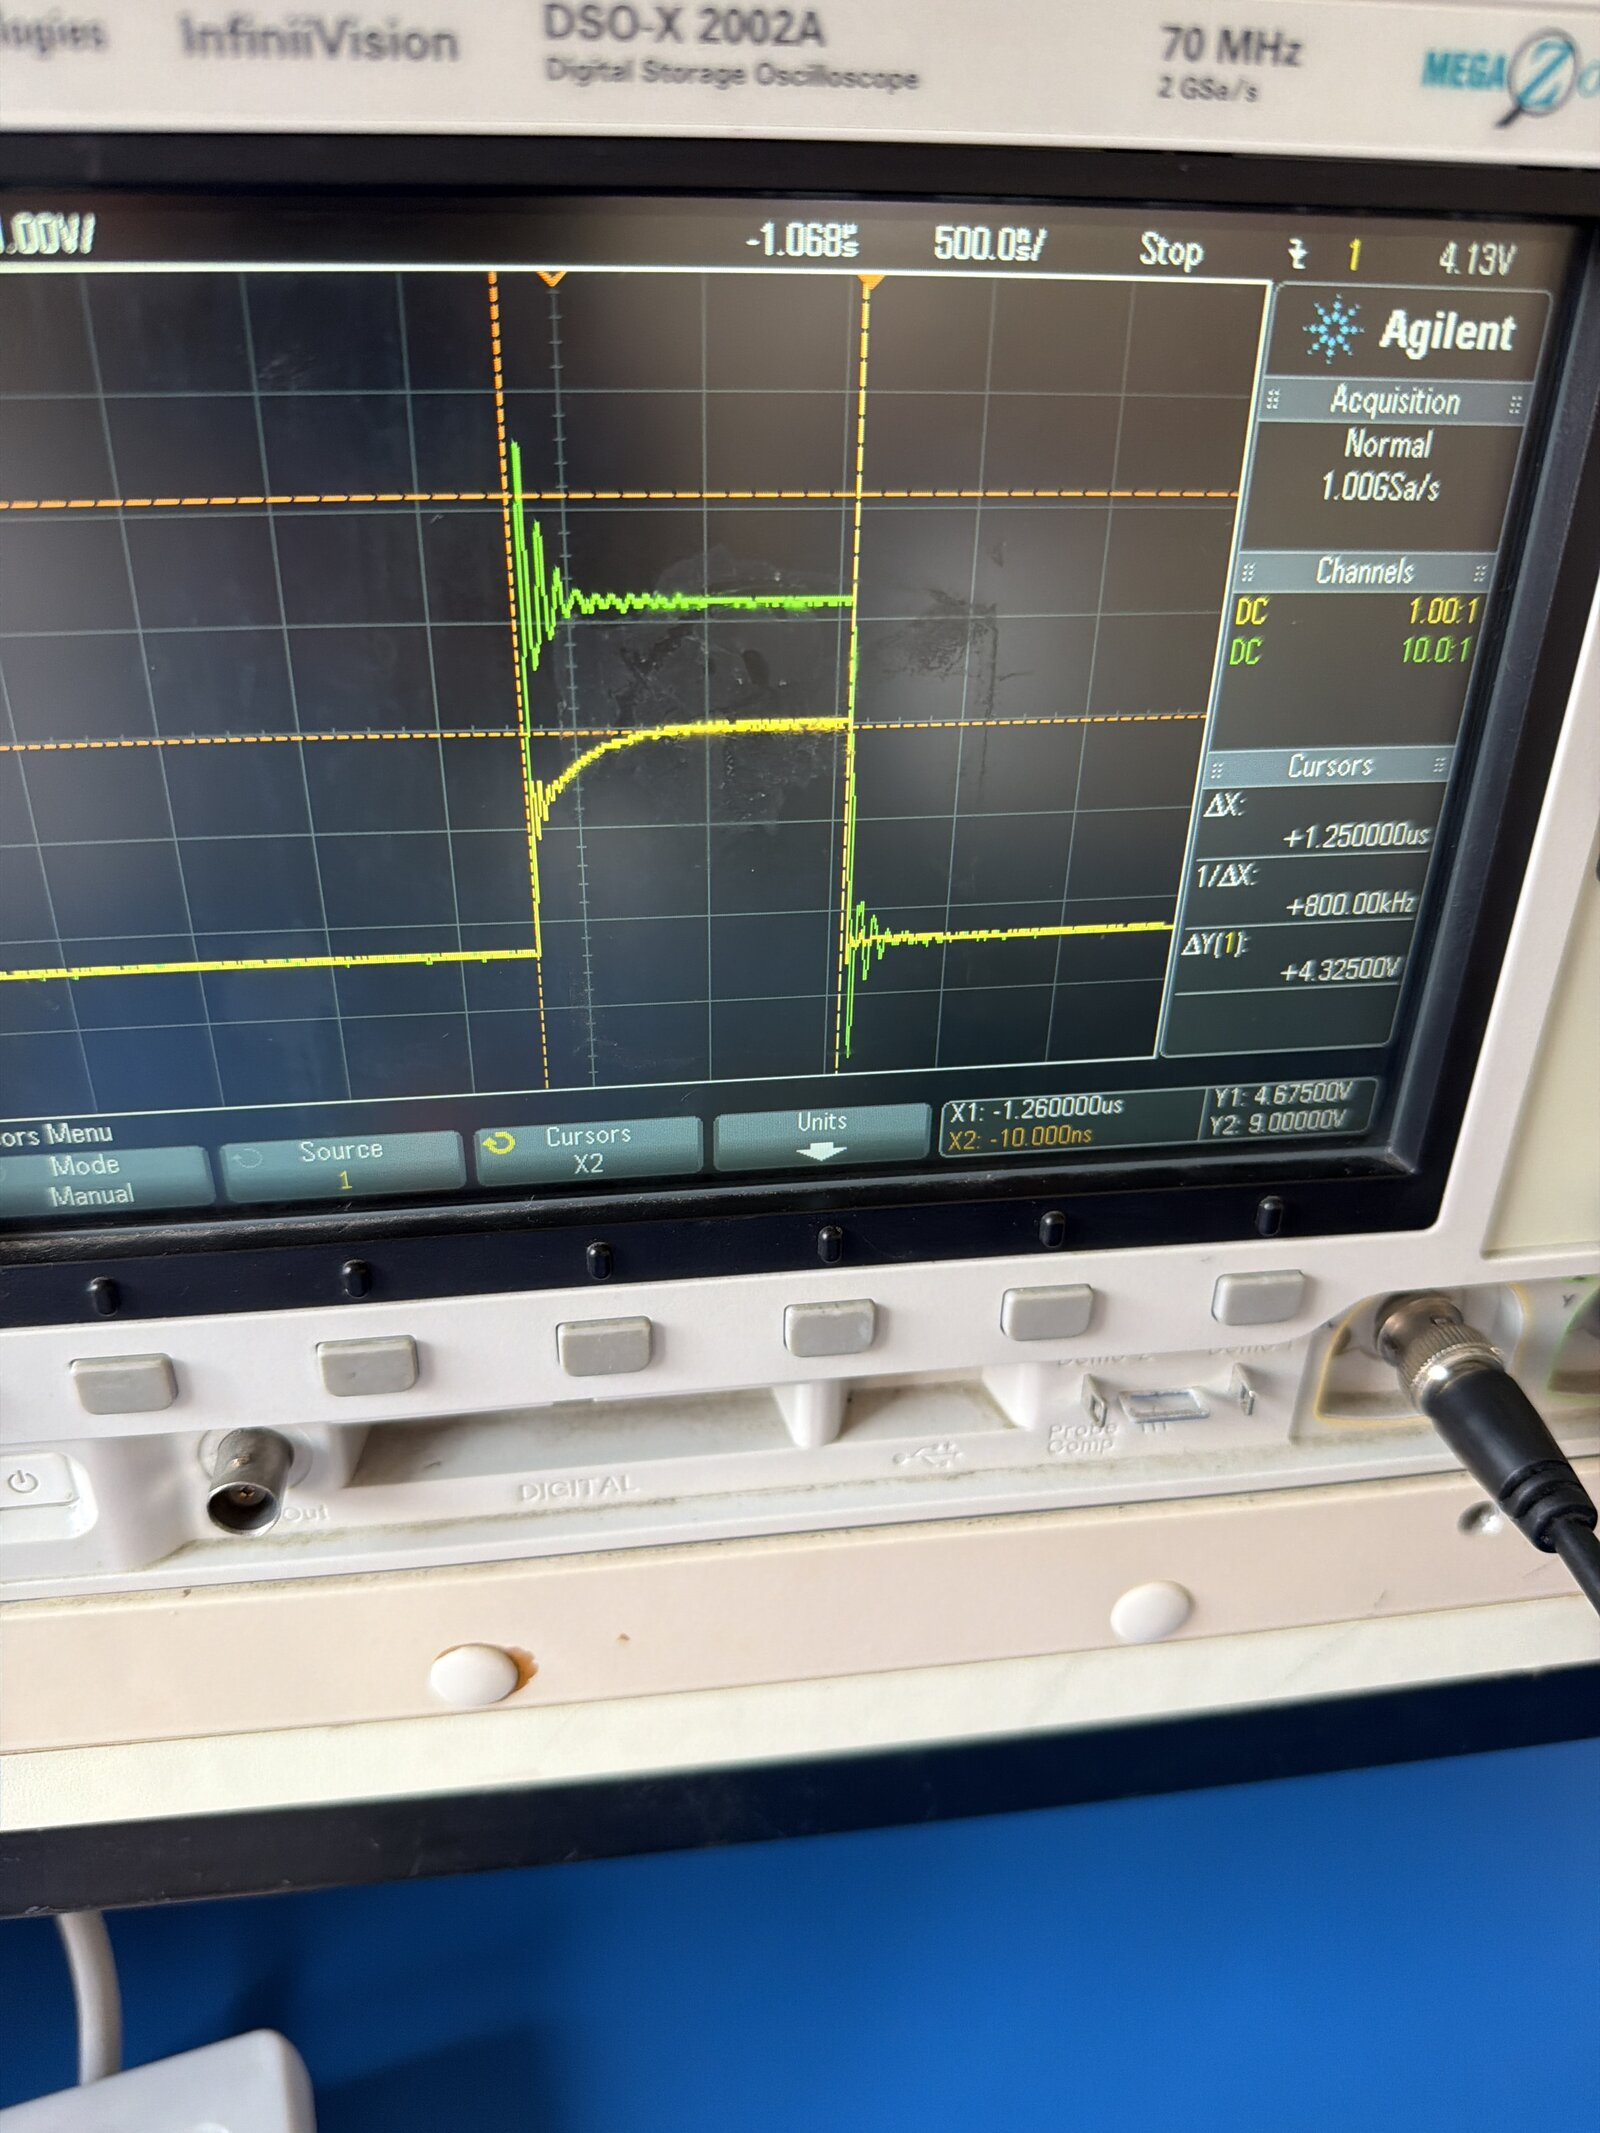
\includegraphics[width=0.62\linewidth]{figures/task5-enable-width-cursors.jpg}
\caption{Horizontal cursors on the corrected Enable pulse measure a total
high time of 1.250 $\mu$s. After subtracting the 220 ns required to reach
3.5 V, the signal remains above the LCD logic-high threshold for approximately
1.030 $\mu$s, exceeding the 450 ns minimum requirement.}
\label{fig:ewidth}
\end{figure}

\subsection{Final result}

With the eight NOP pulse, \texttt{PC15\_S} reached 4.87 V and remained above
3.5 V for longer than the minimum interval specified by the HD44780. The LCD
was successfully initialised in 4 bit mode and displayed the character
\texttt{A} in the first column of the first line. See Figure 15 for evidence.

The loan board's ability to reach nearly 5 V is explained by the 5 V pull-up
on the shifted side of the NMOS level shifter. It is not evidence that the
STM32 output pin itself produced 5 V. The measured \texttt{PC15} level remained
approximately 3.60 V, while the electrically separate \texttt{PC15\_S} node
was charged from the 5 V supply.

\begin{figure}[H]
\centering
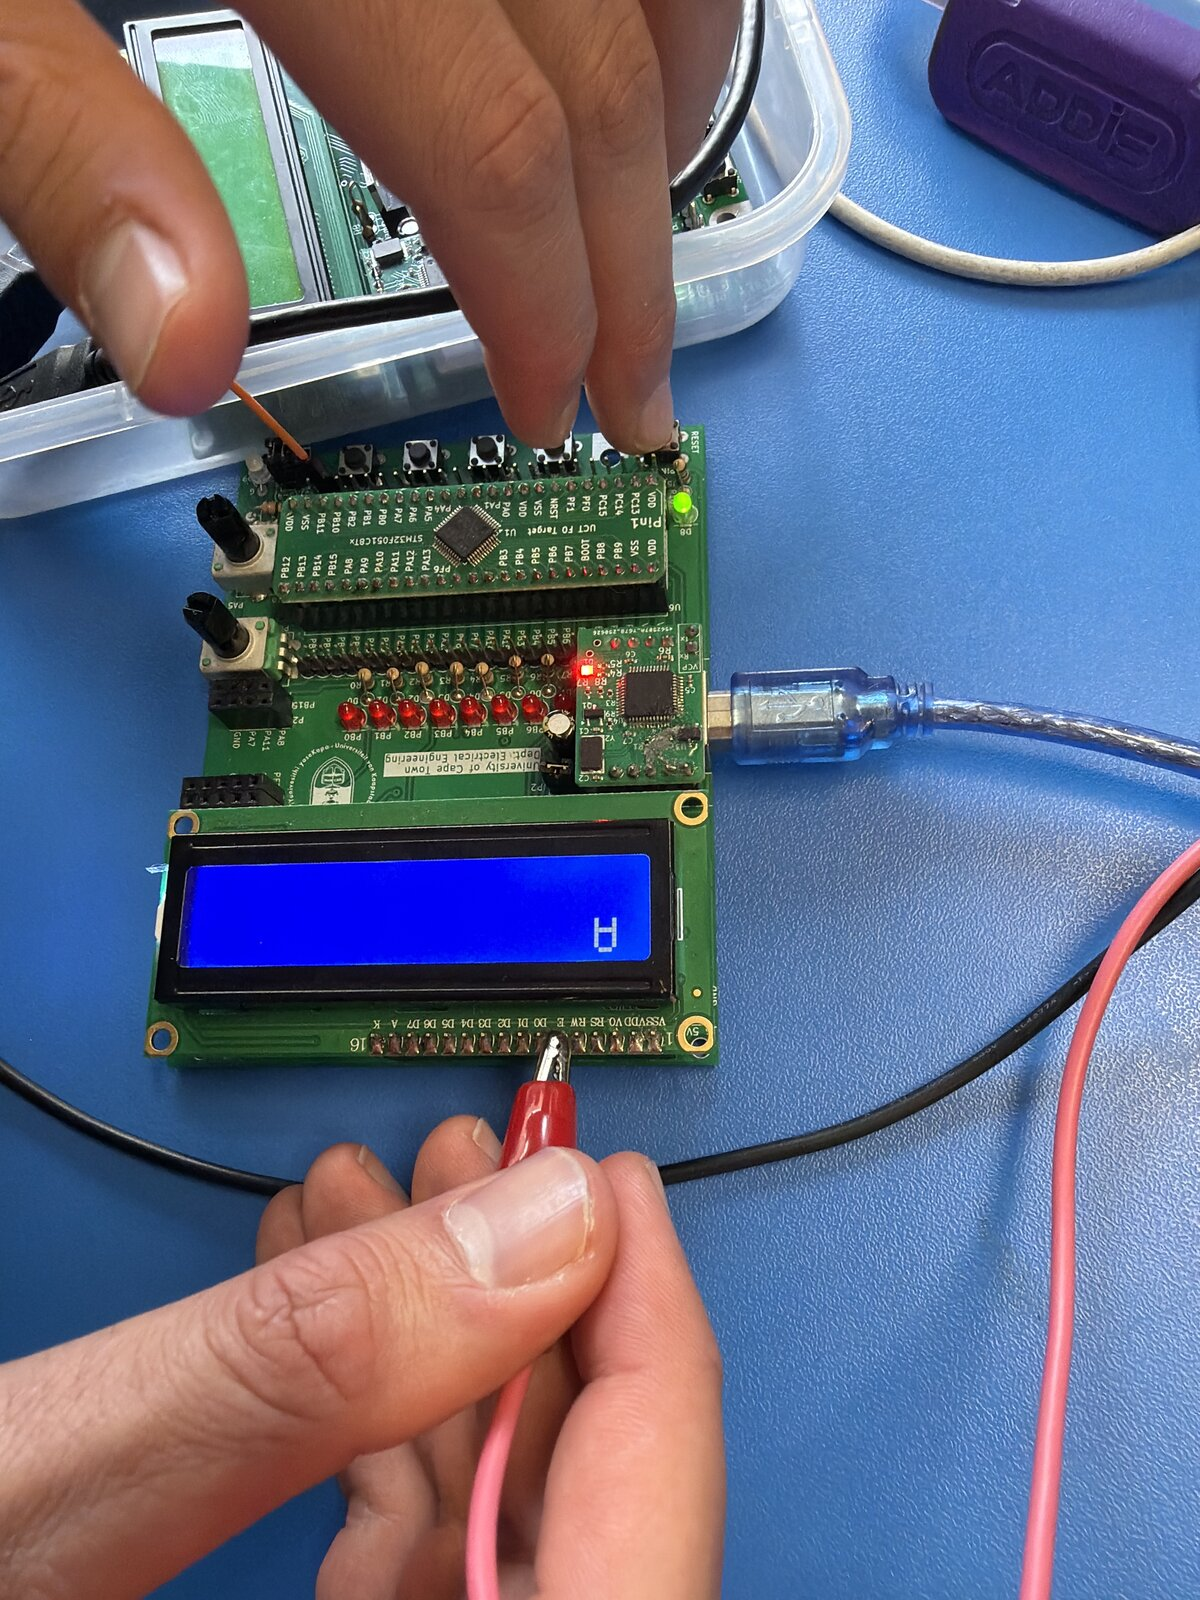
\includegraphics[width=0.58\linewidth]{figures/task5-lcd-photo.jpg}
\caption{Final practical result: the LCD initialised and driven by the
assembly routine, displaying the character \texttt{A} in the first position
of the first line.}
\label{fig:lcd}
\end{figure}
\section*{References}

\begin{itemize}
  \item STMicroelectronics. (2017). \textit{RM0091 Reference manual: STM32F0x1/STM32F0x2/STM32F0x8 advanced ARM-based 32-bit MCUs}. Section 6, Reset and clock control, including Figure 11 clock tree on page 95 and Section 7.2.2 HSI clock on page 98. Section 13, Analog-to-digital converter. Section 14, Digital-to-analog converter. Section 18, General-purpose timers TIM2/TIM3.
  \item STMicroelectronics. (2017). \textit{STM32F051x4 STM32F051x6 STM32F051x8 datasheet}. Pin definitions and ADC characteristics.
  \item Hitachi. \textit{HD44780U (LCD-II) Dot Matrix Liquid Crystal Display Controller/Driver datasheet}. Bus timing characteristics, enable pulse width.
  \item ARM. \textit{Cortex-M0 Technical Reference Manual}. Instruction set summary and cycle counts.
  \item Gowans, J., \& Pead, J. (2025). \textit{UCT Dev Board schematic and pinout reference}, revision 1.06. University of Cape Town.
\end{itemize}

\section*{Appendix: Code}

All source is in the group repository under \texttt{Practical\_1B}. The
listings below are pulled straight from those files when the report is built,
so what is printed here is what was compiled and run.

\subsection*{\texttt{Task1\_PC/golden.c}, Task 1}
\lstinputlisting[language=C]{Task1_PC/golden.c}

\subsection*{\texttt{Task1\_PC/verify\_fast.c}, the cross check}
\lstinputlisting[language=C]{Task1_PC/verify_fast.c}

\subsection*{\texttt{board/Core/Src/main.c}, Tasks 2 and 3}
\lstinputlisting[language=C]{board/Core/Src/main.c}

\subsection*{\texttt{board/Core/Src/phase\_delay.s}, Task 4}
\lstinputlisting{board/Core/Src/phase_delay.s}

\subsection*{\texttt{board/Core/Src/lcd\_asm.s}, Task 5}
\lstinputlisting{board/Core/Src/lcd_asm.s}

\end{document}
